\documentclass[12pt,a4paper]{article}

% Packages essentiels
\usepackage[utf8]{inputenc}
\usepackage[T1]{fontenc}
\usepackage[french]{babel}
\usepackage{geometry}
\geometry{margin=2.5cm, headheight=14.5pt}
\usepackage{graphicx}
\usepackage{hyperref}
\usepackage{cite}
\usepackage{amsmath}
\usepackage{amssymb}
\usepackage{fancyhdr}
\usepackage{titlesec}
\usepackage{multirow}
\usepackage{tabularx}
\usepackage{ragged2e}
\usepackage{float}
\usepackage{tikz}
\usetikzlibrary{arrows.meta, shapes, positioning}
\usepackage{booktabs}
\usepackage{xcolor}
\usepackage{enumitem}
\usepackage{array}
\usepackage{caption}
\usepackage{subcaption}

% Couleurs
\definecolor{headerblue}{RGB}{45, 62, 80}
\definecolor{rowgray}{RGB}{245, 245, 245}
\definecolor{accentblue}{RGB}{0, 80, 136}
\definecolor{qwenred}{RGB}{231, 76, 60}
\definecolor{llamablue}{RGB}{52, 152, 219}
\definecolor{mistralgreen}{RGB}{46, 204, 113}

% Colonne type
\newcolumntype{L}{>{\RaggedRight\arraybackslash}X}
\newcolumntype{C}{>{\centering\arraybackslash}p}

% Configuration des sections
\titleformat{\section}{\Large\bfseries}{\thesection}{1em}{}

% Liens
\hypersetup{
    colorlinks=true,
    linkcolor=accentblue,
    citecolor=accentblue,
    urlcolor=accentblue
}

% En-t\^etes
\pagestyle{fancy}
\fancyhf{}
\fancyhead[L]{\small Universit\'e Toulouse III -- Paul Sabatier}
\fancyhead[R]{\small Master 2 Intelligence Artificielle}
\fancyfoot[C]{\thepage}
\renewcommand{\headrulewidth}{0.4pt}
\renewcommand{\footrulewidth}{0.4pt}

\fancypagestyle{plain}{
    \fancyhf{}
    \fancyfoot[C]{\thepage}
    \renewcommand{\headrulewidth}{0pt}
    \renewcommand{\footrulewidth}{0pt}
}

% Chemin des figures
\graphicspath{{results/Phase2a/}{results/Phase2b/}{results/Phase2c/}{results/Phase2d/}{./}}

\begin{document}

% ============================================================================
% PAGE DE GARDE
% ============================================================================
\begin{titlepage}
    \centering
    
\includegraphics[width=6cm]{logo-UT-site.png}\\[1.5cm]
    {\huge\bfseries Un Syst\`eme Question-R\'eponse\\en G\'eographie\par}
    \vspace{0.5cm}
    {\Large Phase 2 --- Comparaison Multi-LLMs\par}
    \vspace{0.3cm}
    {\large Projet GeoR2LLMs\par}
    \vspace{2cm}
    \begin{minipage}{0.8\textwidth}
        \centering
        \textbf{R\'ealis\'e par :}\\[0.3cm]
        Hiba L'MOUDDEN \\
        Feras MAKHLOUF \\
        Osama BAAZZI \\
        Mohamed DIALLO \\
        Ousama BOUTEZROUT
    \end{minipage}\\[2cm]
    \textbf{Sous la direction de :}\\[0.3cm]
    Lynda TAMINE-LECHANI\\
    IRIT -- Institut de Recherche en Informatique de Toulouse\\[2cm]
    \vfill
    {\large Master 2 Intelligence Artificielle\\
    Universit\'e Toulouse III -- Paul Sabatier\\[0.5cm]
    Ann\'ee universitaire 2024--2025\par}
\end{titlepage}

\newpage
\tableofcontents
\newpage

% ============================================================================
% 1. INTRODUCTION
% ============================================================================
\section{Introduction}

Ce rapport pr\'esente les r\'esultats de la \textbf{Phase~2} du projet GeoR2LLMs, dont l'objectif est de comparer les performances de plusieurs mod\`eles de langue (LLMs) de petite taille dans une configuration de g\'en\'eration augment\'ee par recherche d'information (RAG) pour la question-r\'eponse g\'eographique.

La Phase~1~\cite{huang_geosqa_2019} avait \'etabli un pipeline RAG de r\'ef\'erence avec un seul mod\`ele (Qwen3-0.6B) sur le dataset GeoSQA, r\'ev\'elant des performances limit\'ees (accuracy proche du hasard) et un retrieval quasi-inexistant. La Phase~2 \'etend cette \'evaluation \`a \textbf{5~LLMs} sur \textbf{3~datasets} g\'eographiques distincts pour r\'epondre aux questions suivantes~:

\begin{enumerate}[leftmargin=*]
    \item \textbf{Quel mod\`ele est le plus performant} pour le QA g\'eographique avec RAG~?
    \item \textbf{Quel est l'impact du RAG} sur les performances par rapport au baseline (LLM seul)~?
    \item \textbf{La taille du mod\`ele} est-elle corr\'el\'ee aux performances~?
    \item \textbf{Les r\'esultats sont-ils coh\'erents} entre diff\'erents types de benchmarks~?
\end{enumerate}

% ============================================================================
% 2. M\'ETHODOLOGIE
% ============================================================================
\section{M\'ethodologie}

\subsection{Mod\`eles \'evalu\'es}

Cinq LLMs de petite taille (0.6B \`a 3B param\`etres) ont \'et\'e s\'electionn\'es, couvrant trois familles distinctes (Tableau~\ref{tab:modeles}).

\begin{table}[H]
\centering
\caption{Mod\`eles LLM \'evalu\'es dans la Phase~2.}
\label{tab:modeles}
\begin{tabular}{llrl}
\toprule
\textbf{Mod\`ele} & \textbf{Famille} & \textbf{Taille} & \textbf{Identifiant HuggingFace} \\
\midrule
Qwen3-0.6B & Qwen & 0.6B & \texttt{Qwen/Qwen3-0.6B} \\
Qwen3-1.7B & Qwen & 1.7B & \texttt{Qwen/Qwen3-1.7B} \\
Llama-3.2-1B & Llama & 1.0B & \texttt{meta-llama/Llama-3.2-1B-Instruct} \\
Llama-3.2-3B & Llama & 3.0B & \texttt{meta-llama/Llama-3.2-3B-Instruct} \\
Ministral-3B & Mistral & 3.0B & \texttt{mistralai/Ministral-3-3B-Instruct-2512} \\
\bottomrule
\end{tabular}
\end{table}

\textbf{Note~:} Ministral-3B utilise une configuration \texttt{Mistral3Config} non support\'ee par \texttt{AutoModelForCausalLM} de la biblioth\`eque Transformers. Ce mod\`ele n'a donc pu \^etre \'evalu\'e sur aucun des trois datasets. Seuls \textbf{4~mod\`eles} ont produit des r\'esultats exploitables.

\subsection{Datasets}

Trois benchmarks g\'eographiques de nature diff\'erente ont \'et\'e utilis\'es (Tableau~\ref{tab:datasets}).

\begin{table}[H]
\centering
\caption{Datasets utilis\'es pour l'\'evaluation.}
\label{tab:datasets}
\begin{tabular}{lccll}
\toprule
\textbf{Dataset} & \textbf{Questions} & \textbf{Langue} & \textbf{T\^ache} & \textbf{Corpus RAG} \\
\midrule
GeoSQA & 200 & ZH $\to$ EN & QCM (A/B/C/D) & Wikipedia FR \\
GKMC & 200 & EN & QCM (A/B/C/D) & Wikipedia FR \\
Tourism-QA & 100 & EN & Recommandation POI & Reviews utilisateurs \\
\bottomrule
\end{tabular}
\end{table}

GeoSQA~\cite{huang_geosqa_2019} contient des questions de raisonnement spatial traduites du chinois. GKMC porte sur des connaissances g\'eographiques g\'en\'erales en anglais. Tourism-QA \'evalue la recommandation de points d'int\'er\^et (POI) \`a partir de requ\^etes touristiques.

\subsection{Architecture RAG commune}

Tous les mod\`eles partagent la m\^eme architecture RAG (Figure~\ref{fig:pipeline}).

\begin{figure}[H]
\centering
\begin{tikzpicture}[
    node distance=1.2cm and 2cm,
    block/.style={rectangle, draw, rounded corners, minimum height=1cm, minimum width=2.5cm, align=center, font=\small},
    data/.style={rectangle, draw, dashed, minimum height=0.8cm, minimum width=2cm, align=center, font=\small\itshape},
    arrow/.style={-{Stealth[length=3mm]}, thick}
]
    \node[data] (question) {Question};
    \node[block, right=of question, fill=llamablue!20] (retriever) {Retriever\\BGE-m3 + FAISS};
    \node[data, above=0.8cm of retriever] (corpus) {Corpus\\(Wikipedia / Reviews)};
    \node[block, right=of retriever, fill=qwenred!20] (generator) {G\'en\'erateur\\LLM};
    \node[data, right=of generator] (reponse) {R\'eponse};

    \draw[arrow] (question) -- (retriever);
    \draw[arrow] (corpus) -- (retriever);
    \draw[arrow] (retriever) -- node[above, font=\scriptsize] {Top-$k$ docs} (generator);
    \draw[arrow] (question) -- ++(0,-1) -| (generator);
    \draw[arrow] (generator) -- (reponse);
\end{tikzpicture}
\caption{Architecture RAG commune \`a toutes les \'evaluations. Le retriever (BAAI/bge-m3) encode la question et recherche les $k=5$ chunks les plus similaires via FAISS (IndexFlatIP). Le g\'en\'erateur (LLM) produit la r\'eponse \`a partir de la question et du contexte r\'ecup\'er\'e.}
\label{fig:pipeline}
\end{figure}

\subsection{Protocole d'\'evaluation}

Chaque mod\`ele est \'evalu\'e dans deux conditions~:
\begin{itemize}[leftmargin=*]
    \item \textbf{Baseline} --- le LLM seul, sans contexte RAG.
    \item \textbf{RAG} --- le LLM avec le contexte des top-5 documents r\'ecup\'er\'es.
\end{itemize}

Les m\'etriques utilis\'ees sont~:
\begin{itemize}[leftmargin=*]
    \item \textbf{Accuracy (MCQ)} --- pourcentage de lettres correctes (A/B/C/D) pour GeoSQA et GKMC.
    \item \textbf{Accuracy@1} --- le premier POI recommand\'e est-il correct~? (Tourism-QA).
    \item \textbf{F1} --- score F1 au niveau des tokens entre pr\'ediction et v\'erit\'e terrain.
    \item \textbf{Hit Rate@$k$} --- la r\'eponse appara\^it-elle dans les top-$k$ documents r\'ecup\'er\'es~?
    \item \textbf{MRR@5} --- Mean Reciprocal Rank sur les 5 premiers documents.
\end{itemize}

\subsection{Configuration exp\'erimentale}

Les exp\'eriences ont \'et\'e r\'ealis\'ees sur Google Colab avec un GPU NVIDIA Tesla T4 (16~Go VRAM). Les param\`etres communs sont~: graine al\'eatoire $= 42$, top-$k = 5$, taille de chunk $= 512$ tokens, chevauchement $= 50$ tokens, corpus de 300 articles Wikipedia FR (GeoSQA/GKMC) ou reviews utilisateurs (Tourism-QA).


% ============================================================================
% 3. R\'ESULTATS PAR DATASET
% ============================================================================
\section{R\'esultats par dataset}

\subsection{GeoSQA --- Raisonnement spatial}

Le Tableau~\ref{tab:geosqa} pr\'esente les r\'esultats sur GeoSQA (200 questions).

\begin{table}[H]
\centering
\caption{R\'esultats sur GeoSQA (200 questions, chinois $\to$ anglais, corpus Wikipedia FR).}
\label{tab:geosqa}
\begin{tabular}{lcccccc}
\toprule
\textbf{Mod\`ele} & \textbf{Base. Acc} & \textbf{RAG Acc} & \textbf{$\Delta$ Acc} & \textbf{RAG F1} & \textbf{HR@5} & \textbf{MRR@5} \\
\midrule
Qwen3-1.7B & 0.3900 & \textbf{0.3900} & $+$0.0000 & 0.0107 & 0.065 & 0.040 \\
Llama-3.2-3B & 0.3000 & 0.2750 & $-$0.0250 & 0.0025 & 0.065 & 0.040 \\
Qwen3-0.6B & 0.2700 & 0.2650 & $-$0.0050 & 0.0212 & 0.065 & 0.040 \\
Llama-3.2-1B & 0.2100 & 0.2500 & $+$0.0400 & 0.0034 & 0.065 & 0.040 \\
\midrule
Ministral-3B & \multicolumn{6}{c}{\textit{ERREUR --- Mistral3Config non support\'ee}} \\
\bottomrule
\end{tabular}
\end{table}

\textbf{Observations~:}
\begin{itemize}[leftmargin=*]
    \item Qwen3-1.7B domine avec 0.3900 d'accuracy (proche du hasard \`a 0.25 pour un QCM \`a 4 choix).
    \item Le RAG n'am\'eliore aucun mod\`ele significativement. Llama-3.2-1B est le seul \`a progresser l\'eg\`erement ($+$0.04).
    \item Le retrieval est quasi-inexistant~: Hit Rate@5 = 0.065 et MRR@5 = 0.040 pour tous les mod\`eles (m\^eme retriever). Ceci s'explique par le \textbf{mismatch linguistique}~: les questions sont en anglais (traduites du chinois) alors que le corpus Wikipedia est en fran\c{c}ais.
    \item L'Exact Match est \`a 0.0 pour tous les mod\`eles.
\end{itemize}

\begin{figure}[H]
\centering
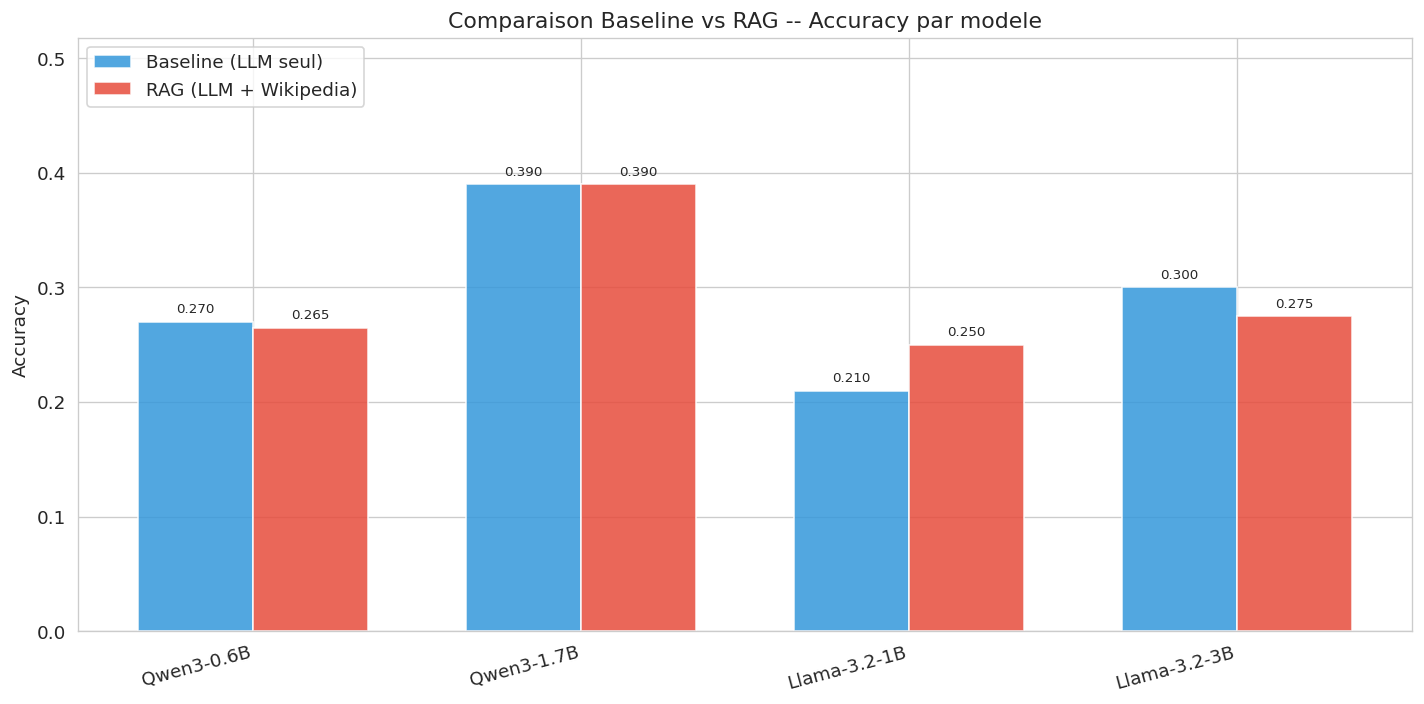
\includegraphics[width=0.85\textwidth]{fig1_accuracy_baseline_vs_rag.png}
\caption{GeoSQA --- Accuracy Baseline vs RAG par mod\`ele.}
\label{fig:geosqa_acc}
\end{figure}

\begin{figure}[H]
\centering
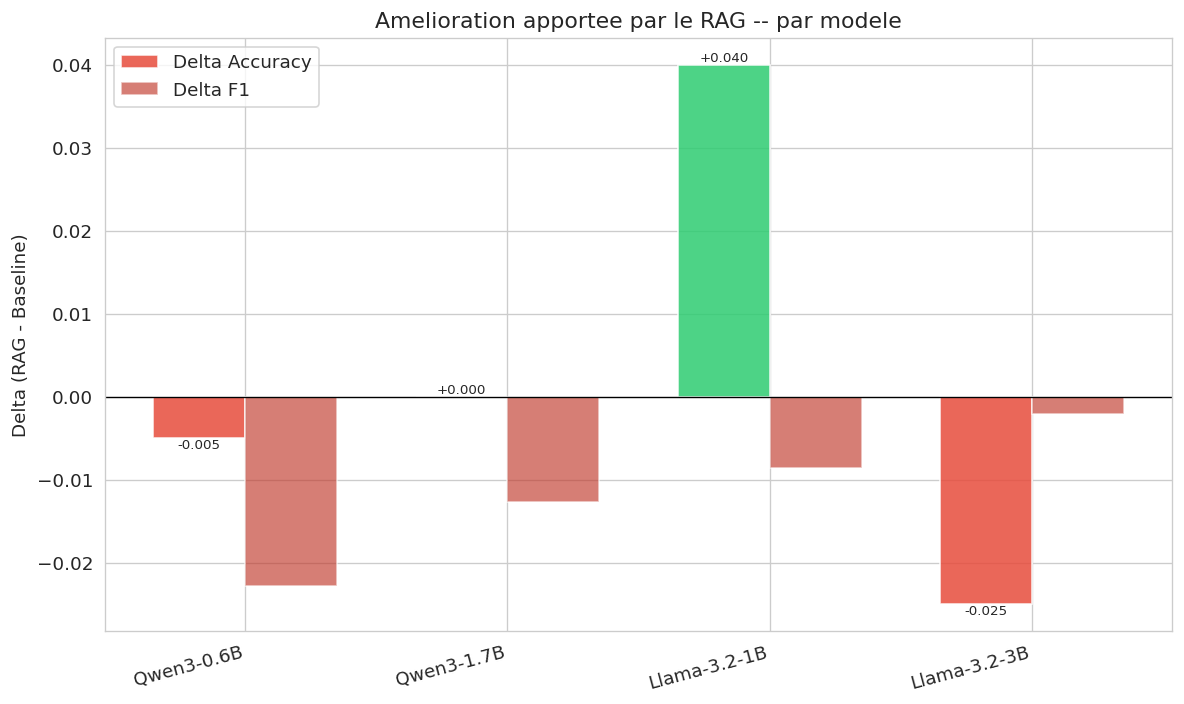
\includegraphics[width=0.85\textwidth]{fig4_improvement_delta.png}
\caption{GeoSQA --- Am\'elioration ($\Delta$) apport\'ee par le RAG.}
\label{fig:geosqa_delta}
\end{figure}


\subsection{GKMC --- Connaissances g\'eographiques g\'en\'erales}

Le Tableau~\ref{tab:gkmc} pr\'esente les r\'esultats sur GKMC (200 questions).

\begin{table}[H]
\centering
\caption{R\'esultats sur GKMC (200 questions, anglais, corpus Wikipedia FR).}
\label{tab:gkmc}
\begin{tabular}{lcccccc}
\toprule
\textbf{Mod\`ele} & \textbf{Base. Acc} & \textbf{RAG Acc} & \textbf{$\Delta$ Acc} & \textbf{RAG F1} & \textbf{HR@5} & \textbf{MRR@5} \\
\midrule
Qwen3-1.7B & 0.5900 & \textbf{0.6100} & $+$0.0200 & 0.0216 & 0.075 & 0.046 \\
Llama-3.2-3B & 0.5200 & 0.4750 & $-$0.0450 & 0.0074 & 0.075 & 0.046 \\
Llama-3.2-1B & 0.4000 & 0.3050 & $-$0.0950 & 0.0082 & 0.075 & 0.046 \\
Qwen3-0.6B & 0.3850 & 0.3700 & $-$0.0150 & 0.0218 & 0.075 & 0.046 \\
\midrule
Ministral-3B & \multicolumn{6}{c}{\textit{ERREUR --- Mistral3Config non support\'ee}} \\
\bottomrule
\end{tabular}
\end{table}

\textbf{Observations~:}
\begin{itemize}[leftmargin=*]
    \item Qwen3-1.7B atteint \textbf{0.6100} d'accuracy avec RAG --- le meilleur score de toute la Phase~2. C'est aussi le seul mod\`ele am\'elior\'e par le RAG ($+$0.02).
    \item GKMC est nettement plus facile que GeoSQA~: le meilleur score passe de 0.39 \`a 0.61, car les questions sont en anglais (pas de barri\`ere de traduction du chinois).
    \item Llama-3.2-1B subit la plus forte d\'egradation ($-$0.095), passant de 0.40 \`a 0.305.
    \item Le retrieval reste faible (HR@5 = 0.075, MRR@5 = 0.046) en raison du corpus fran\c{c}ais.
\end{itemize}

\begin{figure}[H]
\centering
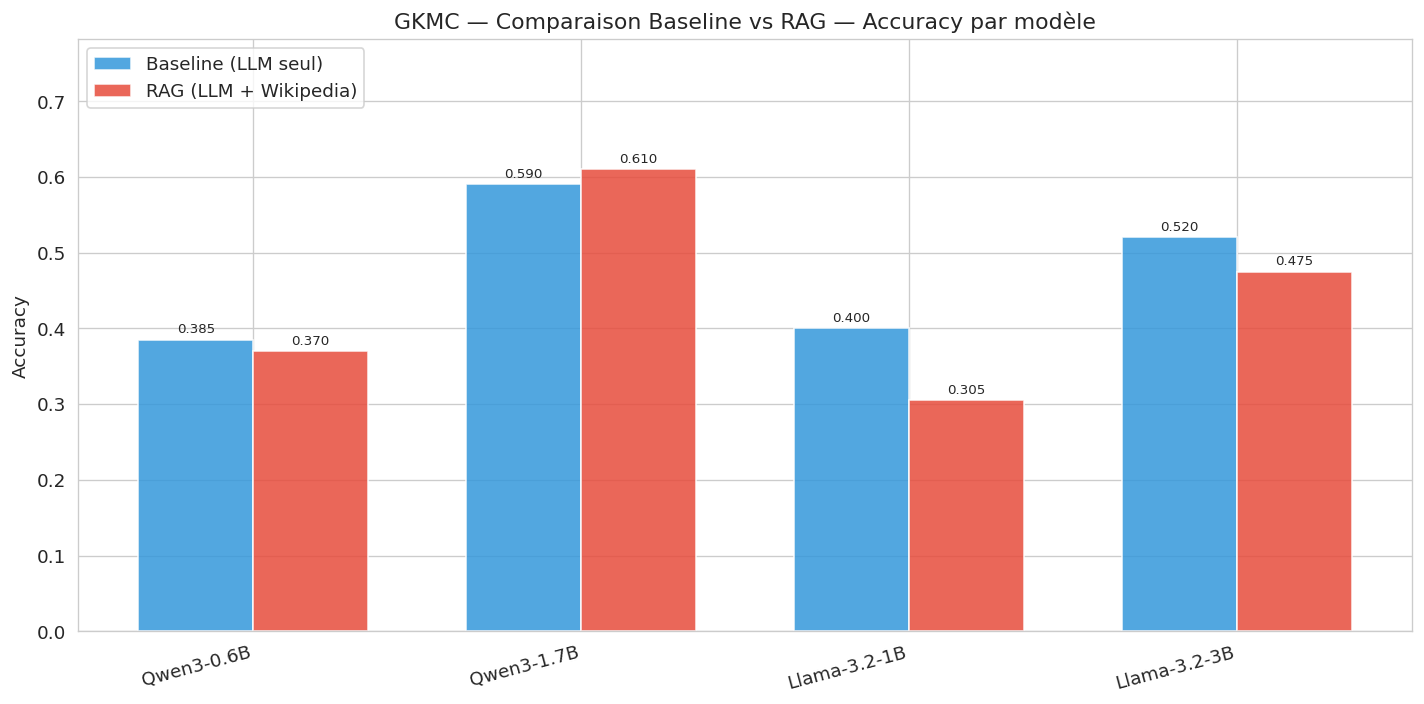
\includegraphics[width=0.85\textwidth]{phase2b_fig1_accuracy_baseline_vs_rag.png}
\caption{GKMC --- Accuracy Baseline vs RAG par mod\`ele.}
\label{fig:gkmc_acc}
\end{figure}

\begin{figure}[H]
\centering
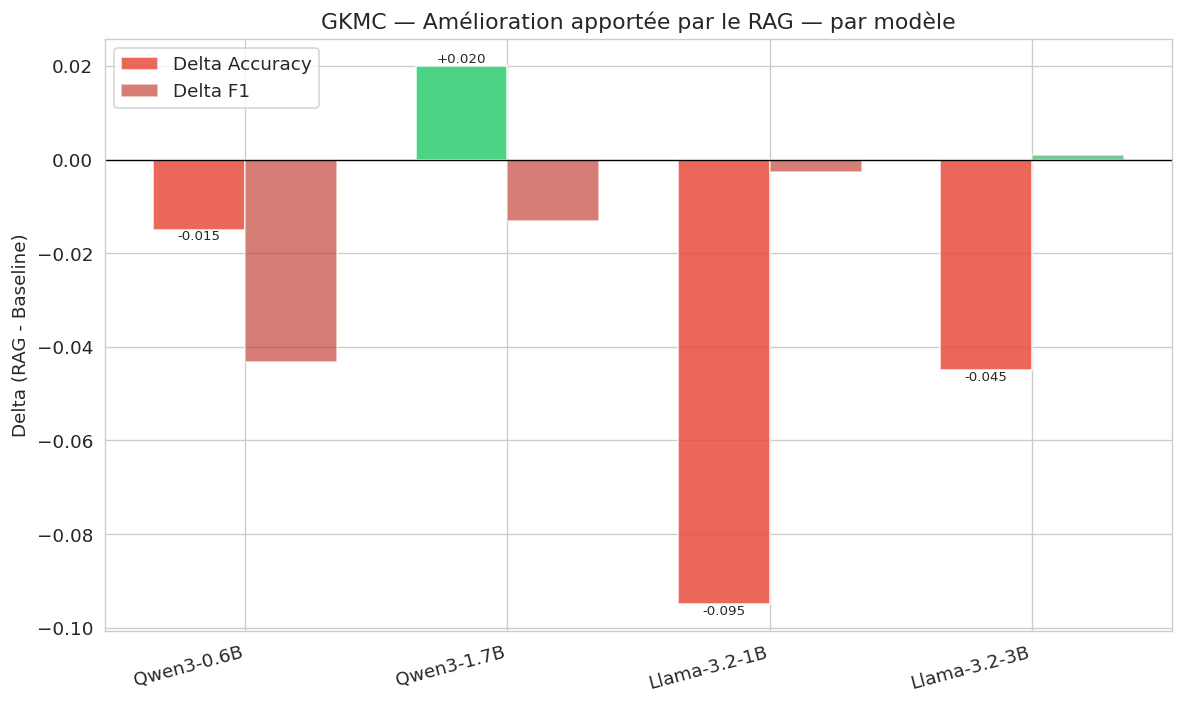
\includegraphics[width=0.85\textwidth]{phase2b_fig4_improvement_delta.png}
\caption{GKMC --- Am\'elioration ($\Delta$) apport\'ee par le RAG.}
\label{fig:gkmc_delta}
\end{figure}


\subsection{Tourism-QA --- Recommandation de POI}

Le Tableau~\ref{tab:tourismqa} pr\'esente les r\'esultats sur Tourism-QA (100 questions).

\begin{table}[H]
\centering
\caption{R\'esultats sur Tourism-QA (100 questions, anglais, corpus de reviews).}
\label{tab:tourismqa}
\begin{tabular}{lccccc}
\toprule
\textbf{Mod\`ele} & \textbf{Base. Acc@1} & \textbf{RAG Acc@1} & \textbf{$\Delta$ Acc@1} & \textbf{RAG F1} & \textbf{Retr. HR} \\
\midrule
Qwen3-0.6B & 0.6000 & \textbf{0.6600} & $+$0.0600 & 0.6464 & 0.48 \\
Llama-3.2-3B & 0.7100 & 0.5900 & $-$0.1200 & 0.5950 & 0.48 \\
Qwen3-1.7B & 0.5800 & 0.5300 & $-$0.0500 & 0.5390 & 0.48 \\
Llama-3.2-1B & 0.4400 & 0.4100 & $-$0.0300 & 0.4033 & 0.48 \\
\midrule
Ministral-3B & \multicolumn{5}{c}{\textit{ERREUR --- Mistral3Config non support\'ee}} \\
\bottomrule
\end{tabular}
\end{table}

\textbf{Observations~:}
\begin{itemize}[leftmargin=*]
    \item R\'esultat surprenant~: \textbf{Qwen3-0.6B} (le plus petit mod\`ele) domine en mode RAG avec 0.6600 d'Acc@1. C'est aussi le seul mod\`ele am\'elior\'e par le RAG ($+$0.06).
    \item En baseline, Llama-3.2-3B est le meilleur (0.7100), mais le RAG le d\'egrade fortement ($-$0.12), le faisant chuter \`a 0.5900.
    \item Le retrieval est bien meilleur que sur GeoSQA/GKMC~: Hit Rate = 0.48 (vs 0.065--0.075). Les reviews sont en anglais, comme les questions, \'eliminant le mismatch linguistique.
    \item Les scores F1 sont beaucoup plus \'elev\'es (0.40--0.65 vs $<$0.05 sur GeoSQA/GKMC) car la t\^ache est diff\'erente (recommandation vs QCM).
\end{itemize}

\begin{figure}[H]
\centering
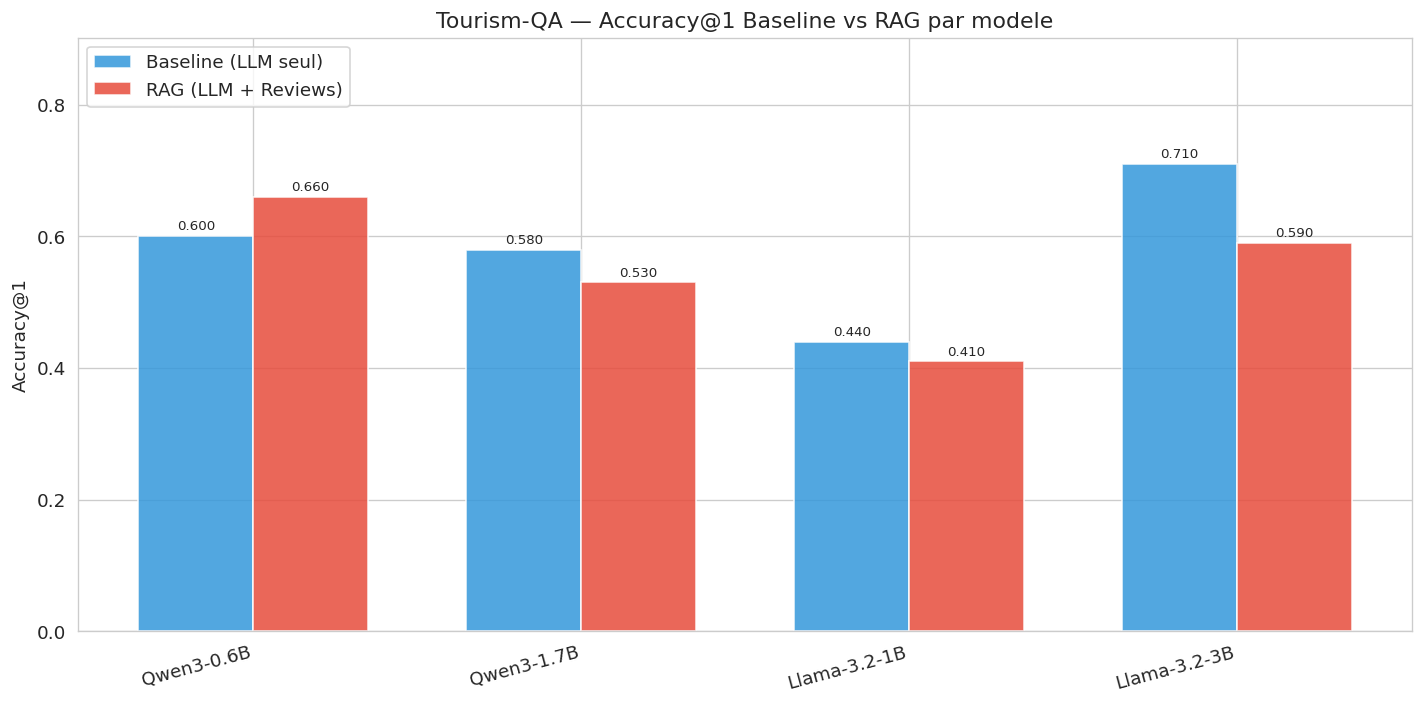
\includegraphics[width=0.85\textwidth]{fig1_poi_accuracy_baseline_vs_rag.png}
\caption{Tourism-QA --- Accuracy@1 Baseline vs RAG par mod\`ele.}
\label{fig:tourism_acc}
\end{figure}

\begin{figure}[H]
\centering
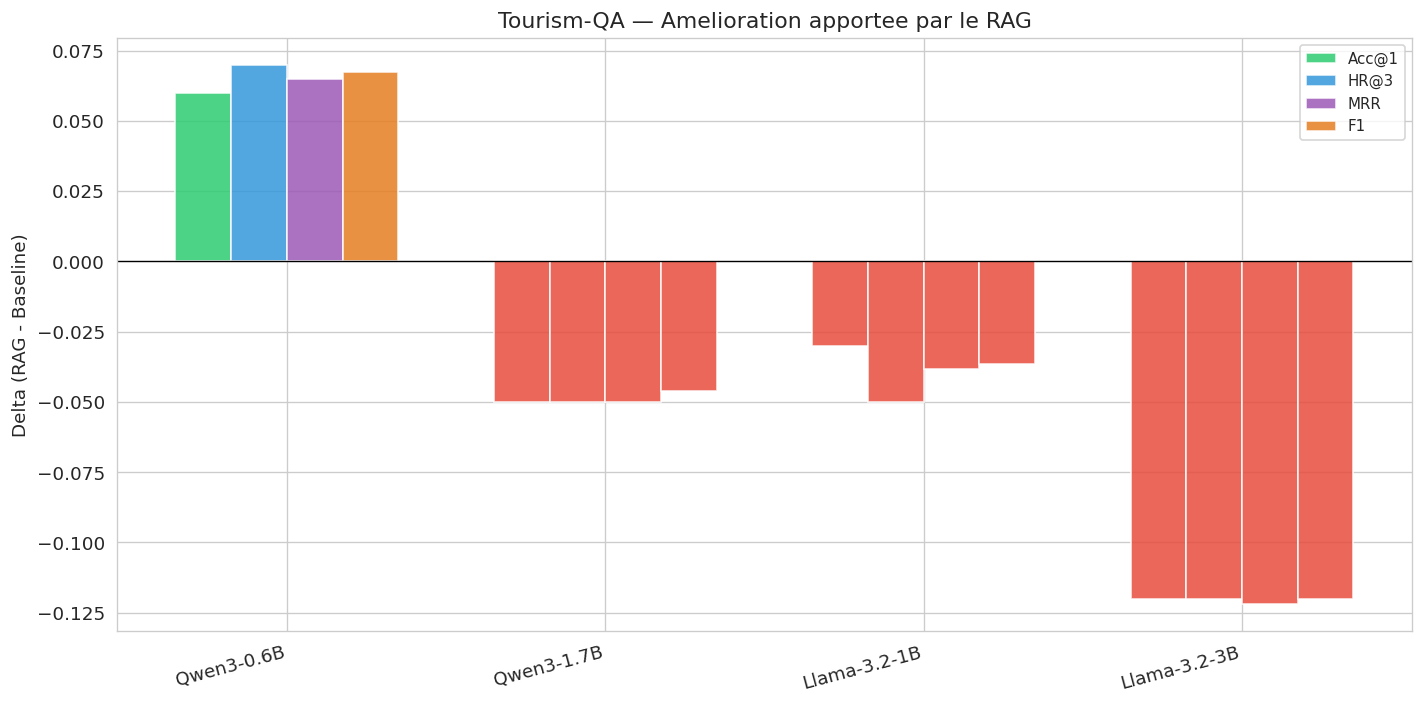
\includegraphics[width=0.85\textwidth]{fig4_poi_improvement_delta.png}
\caption{Tourism-QA --- Am\'elioration ($\Delta$) apport\'ee par le RAG.}
\label{fig:tourism_delta}
\end{figure}


% ============================================================================
% 4. ANALYSE FACTORIELLE CROIS\'EE
% ============================================================================
\section{Analyse factorielle crois\'ee}

La Phase~2d agrège les r\'esultats des trois datasets pour identifier les facteurs d\'eterminants. Le DataFrame unifi\'e contient 12 lignes (4~mod\`eles $\times$ 3~datasets).

\subsection{Effet de la taille du mod\`ele}

La corr\'elation de Pearson entre la taille du mod\`ele et la RAG Accuracy, calcul\'ee sur l'ensemble des 12 configurations, est~:
$$r = 0.19, \quad p = 0.56 \quad \text{(non significatif)}$$

Par dataset~:
\begin{itemize}[leftmargin=*]
    \item GeoSQA~: $r = 0.19$, $p = 0.81$
    \item GKMC~: $r = 0.52$, $p = 0.48$
    \item Tourism-QA~: $r = 0.08$, $p = 0.92$
\end{itemize}

La tendance est positive mais la corr\'elation n'est \textbf{jamais significative}. Les mod\`eles Qwen (0.6B et 1.7B) surpassent syst\'ematiquement les Llama de taille sup\'erieure, montrant que la \textbf{famille du mod\`ele} est un facteur plus d\'eterminant que sa taille.

\begin{figure}[H]
\centering
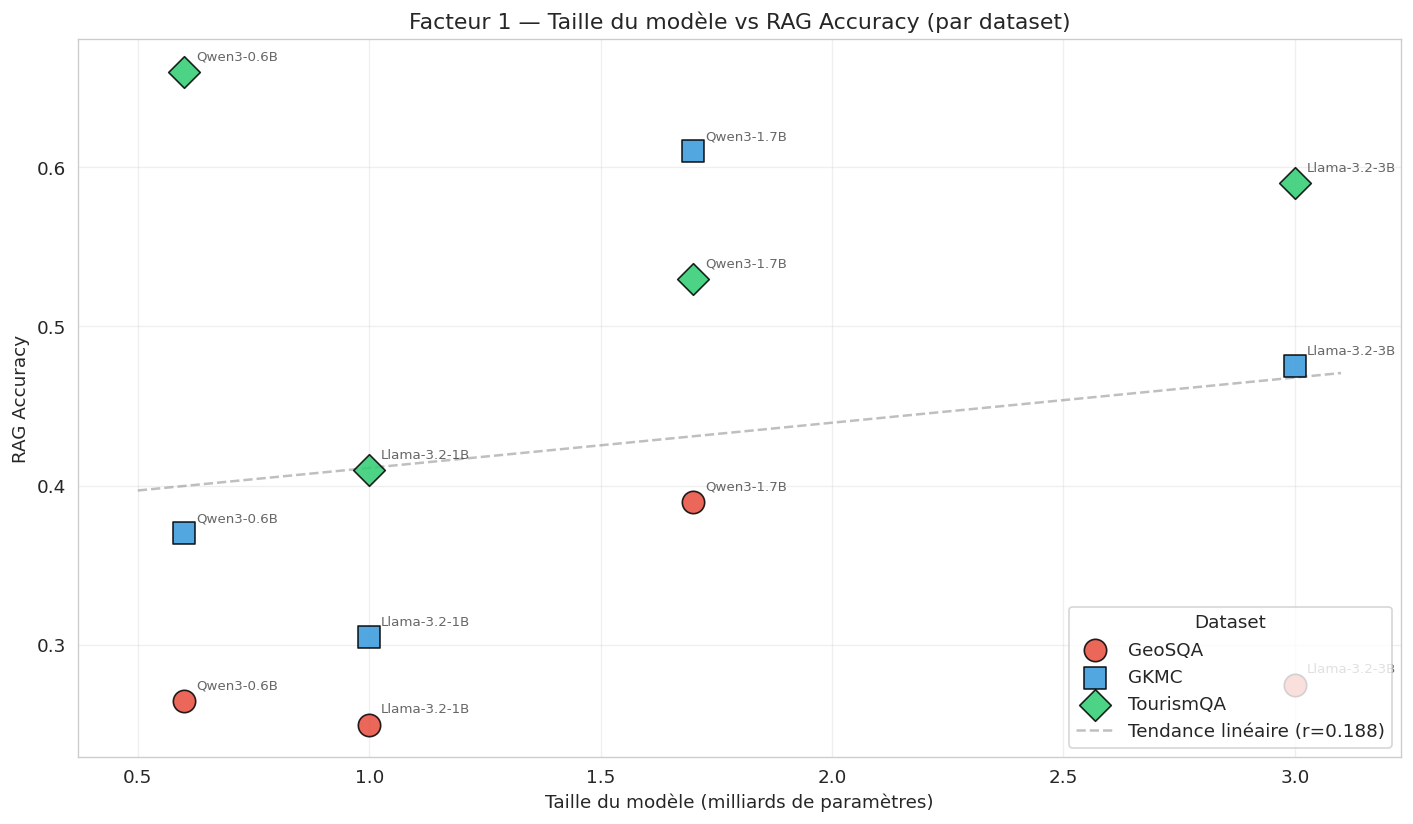
\includegraphics[width=0.85\textwidth]{phase2d_fig1_taille_vs_accuracy.png}
\caption{Taille du mod\`ele vs RAG Accuracy (tous datasets confondus).}
\label{fig:taille}
\end{figure}

\subsection{Effet de la famille}

Qwen surpasse Llama de mani\`ere consistante sur les trois datasets~:

\begin{table}[H]
\centering
\caption{RAG Accuracy moyenne par famille et par dataset.}
\label{tab:famille}
\begin{tabular}{lccc}
\toprule
\textbf{Famille} & \textbf{GeoSQA} & \textbf{GKMC} & \textbf{Tourism-QA} \\
\midrule
Qwen & 0.3275 & 0.4900 & 0.5950 \\
Llama & 0.2625 & 0.3900 & 0.5000 \\
\midrule
$\Delta$ (Qwen $-$ Llama) & $+$0.0650 & $+$0.1000 & $+$0.0950 \\
\bottomrule
\end{tabular}
\end{table}

L'avantage de Qwen est constant ($+$0.065 \`a $+$0.100) quels que soient le dataset et la t\^ache.

\begin{figure}[H]
\centering
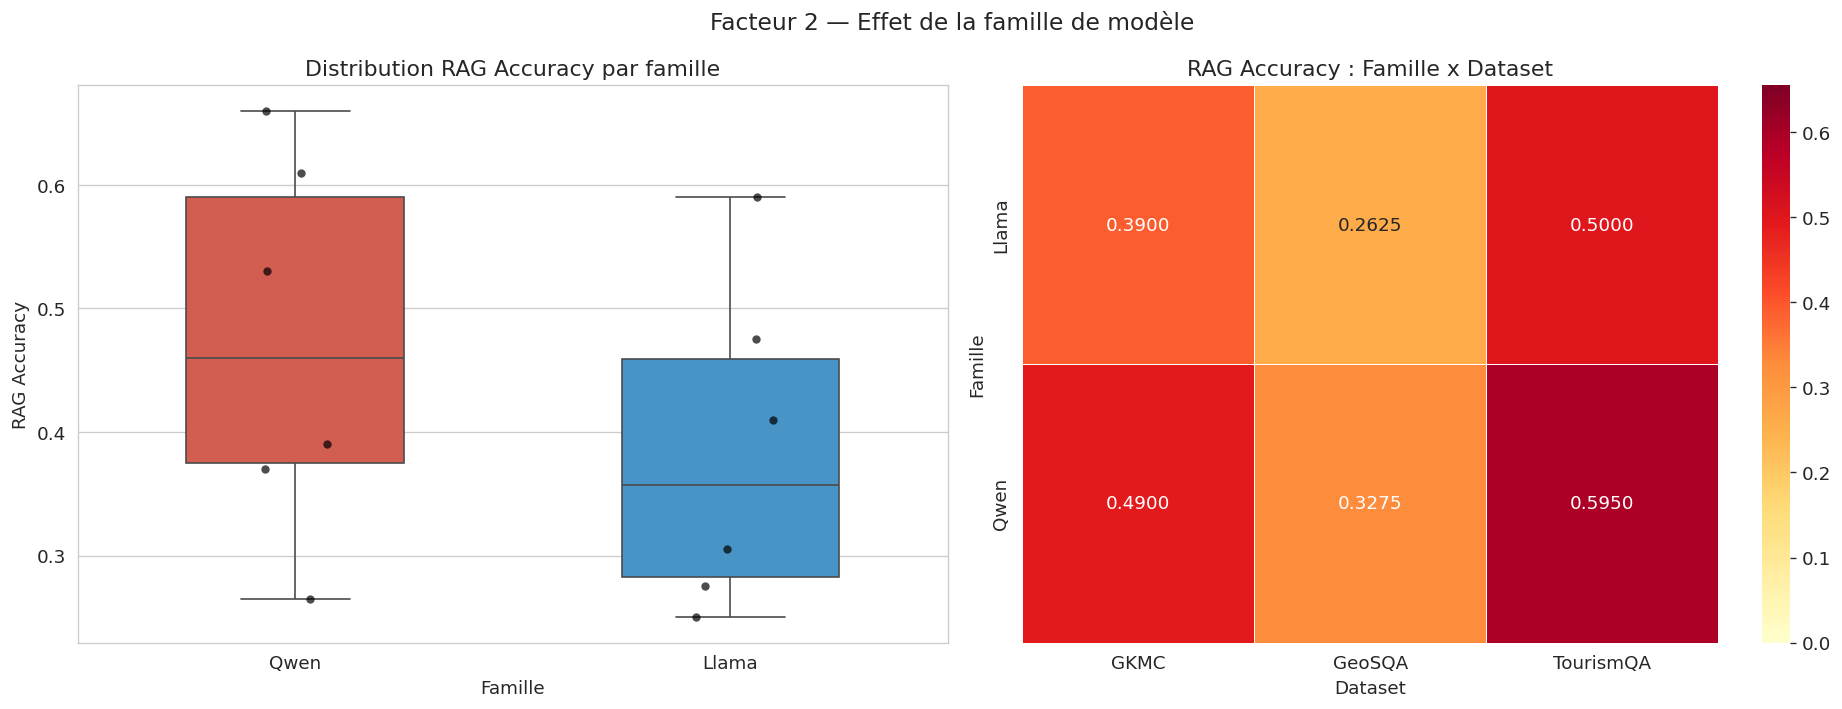
\includegraphics[width=0.85\textwidth]{phase2d_fig2_famille_analyse.png}
\caption{Analyse par famille de mod\`ele.}
\label{fig:famille}
\end{figure}

\subsection{Effet du dataset}

La difficult\'e relative des datasets (mesur\'ee par la RAG Accuracy moyenne) est~:

\begin{table}[H]
\centering
\caption{Difficult\'e des datasets (RAG Accuracy moyenne sur 4 mod\`eles).}
\label{tab:difficulte}
\begin{tabular}{lcc}
\toprule
\textbf{Dataset} & \textbf{RAG Acc moyenne} & \textbf{Classement} \\
\midrule
Tourism-QA & 0.5475 & 1 (plus facile) \\
GKMC & 0.4400 & 2 \\
GeoSQA & 0.2950 & 3 (plus difficile) \\
\bottomrule
\end{tabular}
\end{table}

GeoSQA est le dataset le plus difficile, principalement en raison du mismatch linguistique (questions traduites du chinois, corpus en fran\c{c}ais). Tourism-QA b\'en\'eficie d'un corpus de reviews en anglais, align\'e linguistiquement avec les questions.

\begin{figure}[H]
\centering
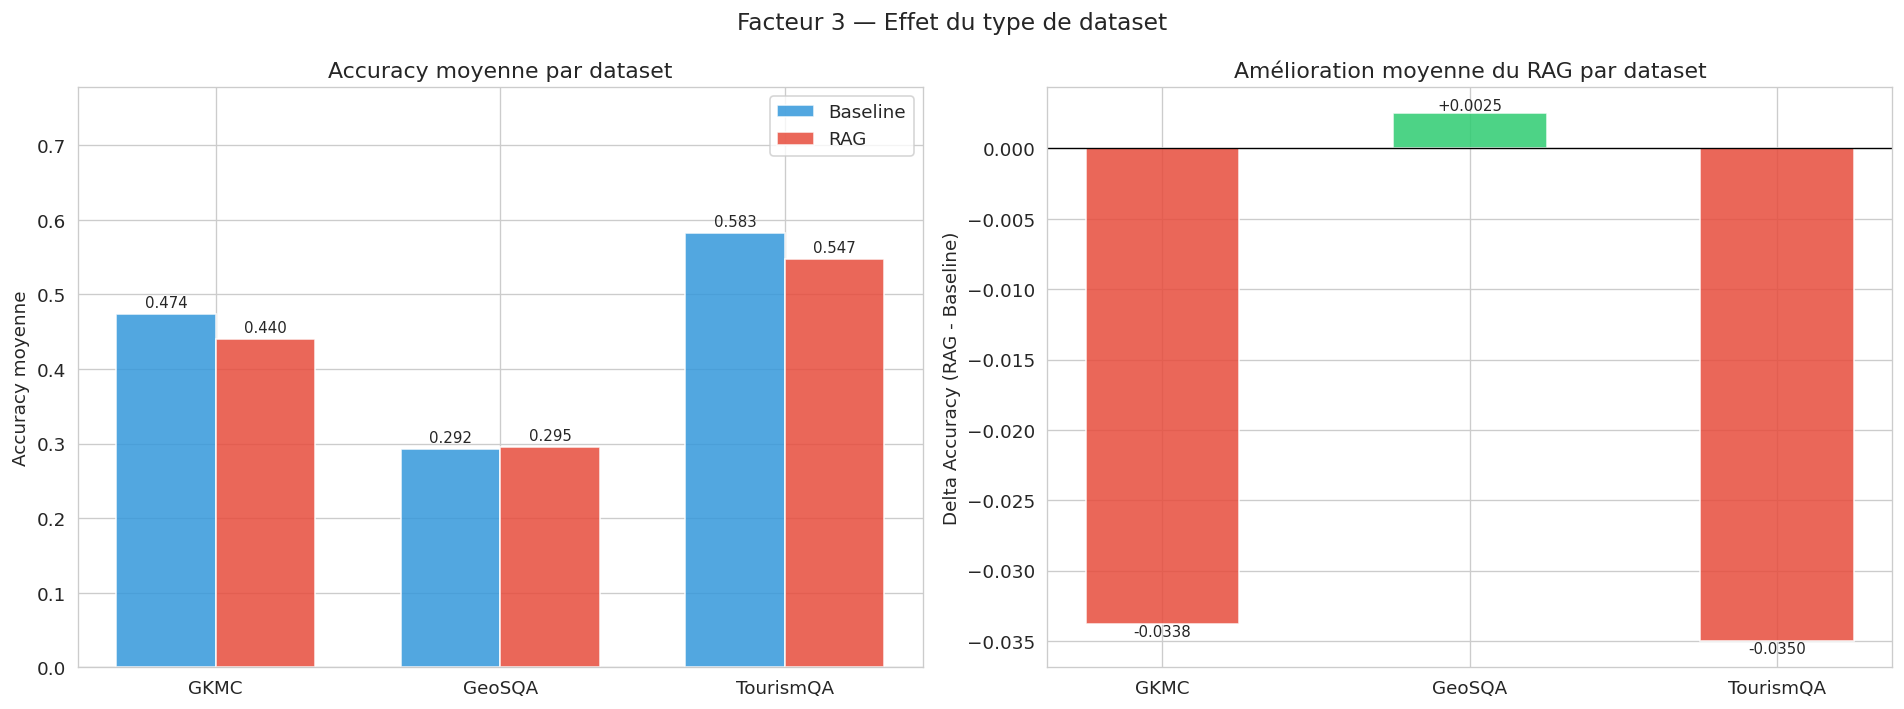
\includegraphics[width=0.85\textwidth]{phase2d_fig3_dataset_analyse.png}
\caption{Analyse par dataset.}
\label{fig:dataset}
\end{figure}

\subsection{Impact du RAG}

L'impact moyen du RAG sur l'accuracy est \textbf{n\'egatif}~: $\Delta = -0.0221$.

\begin{table}[H]
\centering
\caption{Impact du RAG par mod\`ele (moyenne sur 3 datasets).}
\label{tab:rag_impact}
\begin{tabular}{lcc}
\toprule
\textbf{Mod\`ele} & \textbf{$\Delta$ Acc moyenne} & \textbf{Mod\`eles am\'elior\'es} \\
\midrule
Qwen3-0.6B & $+$0.0133 & 1/3 datasets \\
Qwen3-1.7B & $-$0.0100 & 1/3 datasets \\
Llama-3.2-1B & $-$0.0283 & 1/3 datasets \\
Llama-3.2-3B & $-$0.0633 & 0/3 datasets \\
\midrule
\textbf{Moyenne} & $-$0.0221 & --- \\
\bottomrule
\end{tabular}
\end{table}

Le RAG d\'egrade les performances dans la majorit\'e des cas. Seul Qwen3-0.6B a un $\Delta$ moyen positif ($+$0.0133), grâce \`a son am\'elioration sur Tourism-QA ($+$0.06).

\begin{figure}[H]
\centering
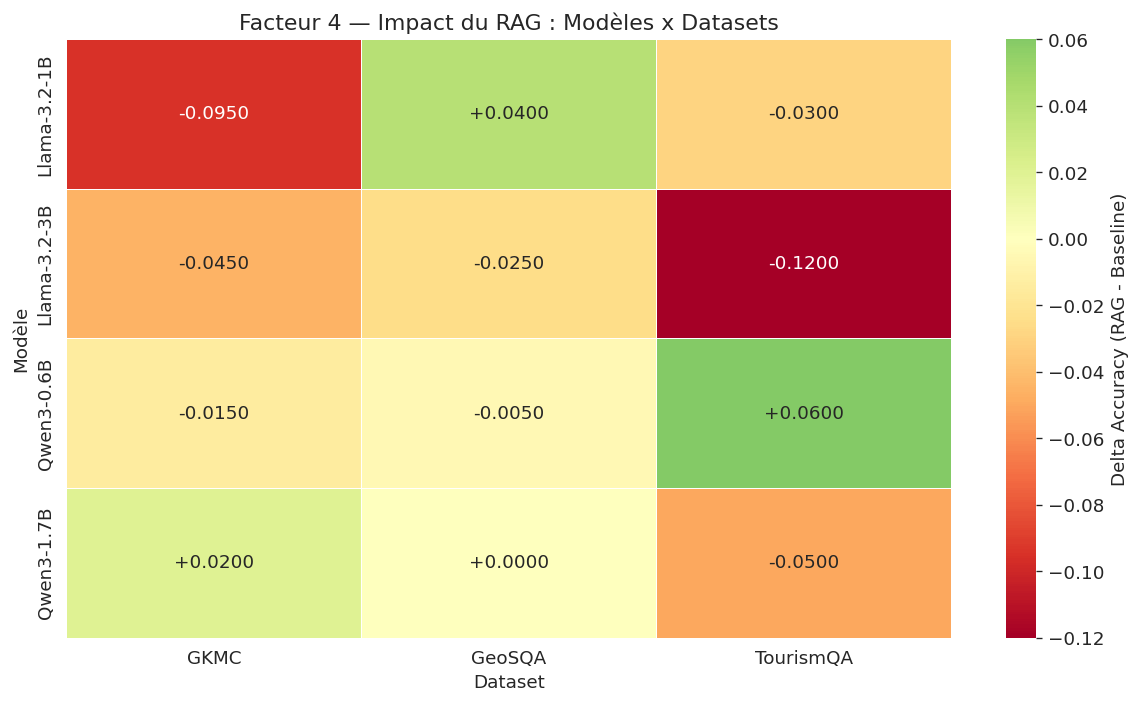
\includegraphics[width=0.85\textwidth]{phase2d_fig4_impact_rag_heatmap.png}
\caption{Heatmap de l'impact du RAG ($\Delta$ Accuracy) par mod\`ele et dataset.}
\label{fig:rag_heatmap}
\end{figure}

\subsection{Classement global}

Le Tableau~\ref{tab:classement} pr\'esente le classement global (moyenne des RAG Accuracy sur les 3 datasets).

\begin{table}[H]
\centering
\caption{Classement global des mod\`eles (moyenne RAG Accuracy sur 3 datasets).}
\label{tab:classement}
\begin{tabular}{clccccc}
\toprule
\textbf{Rang} & \textbf{Mod\`ele} & \textbf{RAG Acc} & \textbf{F1 moy} & \textbf{$\Delta$ moy} & \textbf{$\sigma$} & \textbf{Efficacit\'e} \\
\midrule
1 & Qwen3-1.7B & \textbf{0.5100} & 0.1904 & $-$0.0100 & 0.1114 & 0.3000 \\
2 & Llama-3.2-3B & 0.4467 & 0.2016 & $-$0.0633 & 0.1594 & 0.1489 \\
3 & Qwen3-0.6B & 0.4317 & 0.2298 & $+$0.0133 & 0.2046 & \textbf{0.7195} \\
4 & Llama-3.2-1B & 0.3217 & 0.1383 & $-$0.0283 & 0.0813 & 0.3217 \\
\bottomrule
\end{tabular}
\end{table}

\textbf{Qwen3-1.7B} est le meilleur mod\`ele global avec une RAG Accuracy moyenne de 0.5100. Qwen3-0.6B offre la meilleure \textbf{efficacit\'e} (Accuracy/Taille = 0.7195), ce qui en fait le choix optimal sous contraintes de ressources.

\begin{figure}[H]
\centering
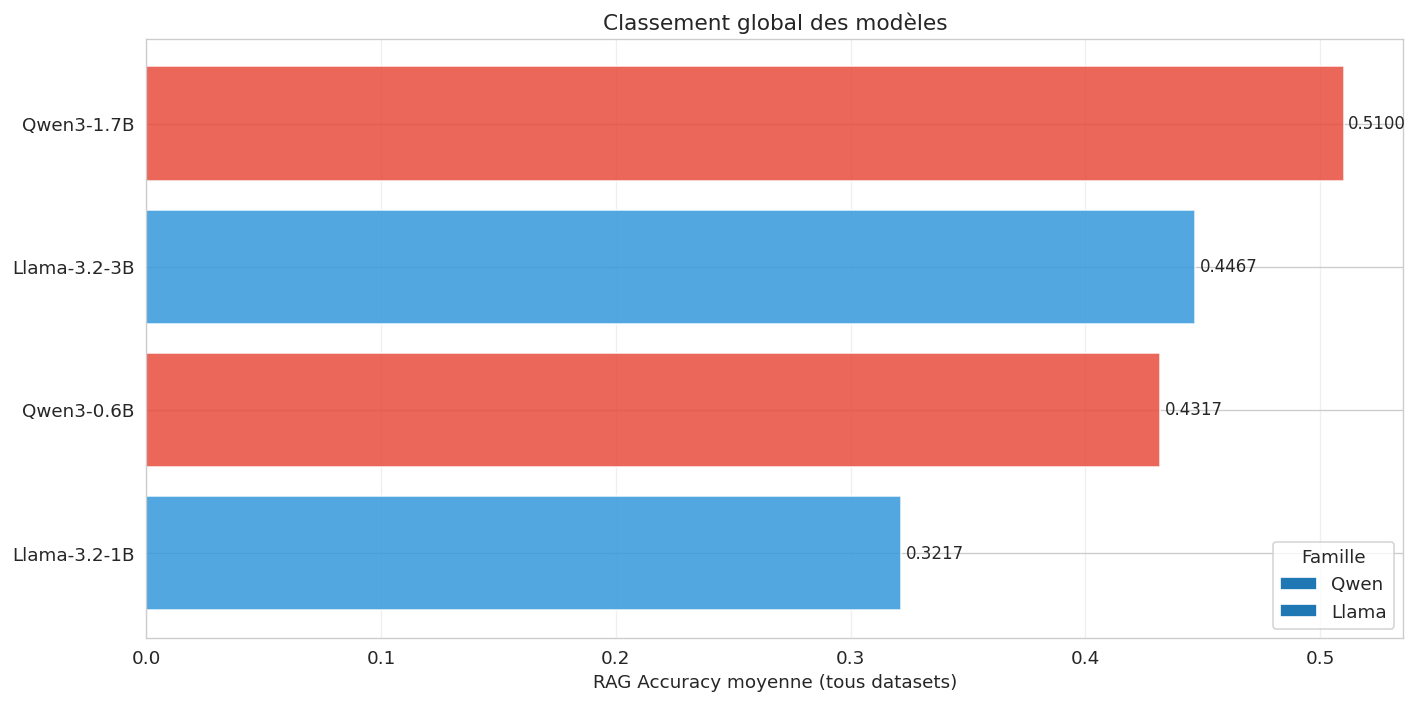
\includegraphics[width=0.85\textwidth]{phase2d_fig9_classement_final.png}
\caption{Classement final des mod\`eles.}
\label{fig:classement}
\end{figure}

\begin{figure}[H]
\centering
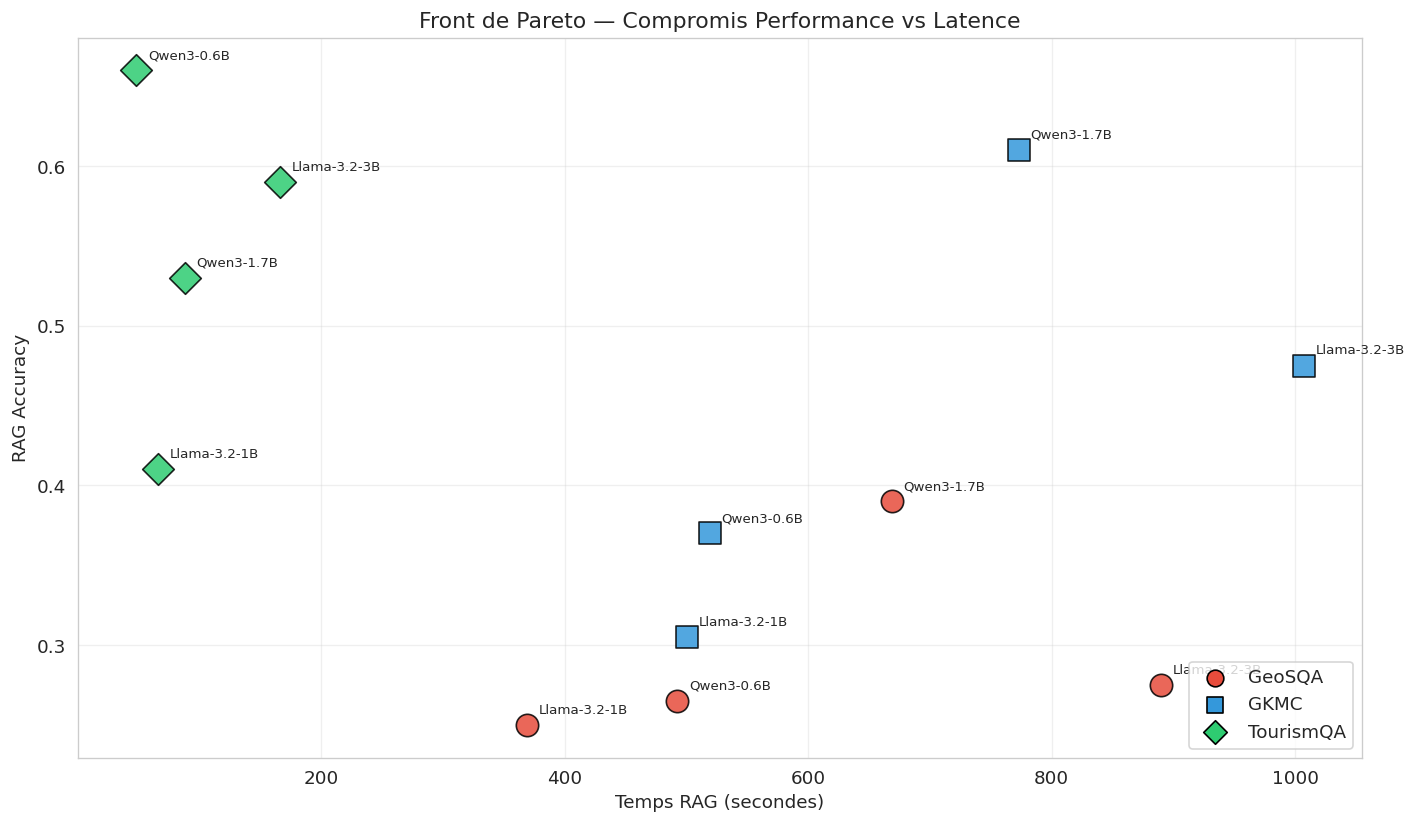
\includegraphics[width=0.85\textwidth]{phase2d_fig8_pareto.png}
\caption{Front de Pareto --- Compromis performance/taille.}
\label{fig:pareto}
\end{figure}

\subsection{Heatmap crois\'ee}

La Figure~\ref{fig:heatmap} donne une vue d'ensemble de toutes les m\'etriques RAG pour chaque combinaison mod\`ele $\times$ dataset.

\begin{figure}[H]
\centering
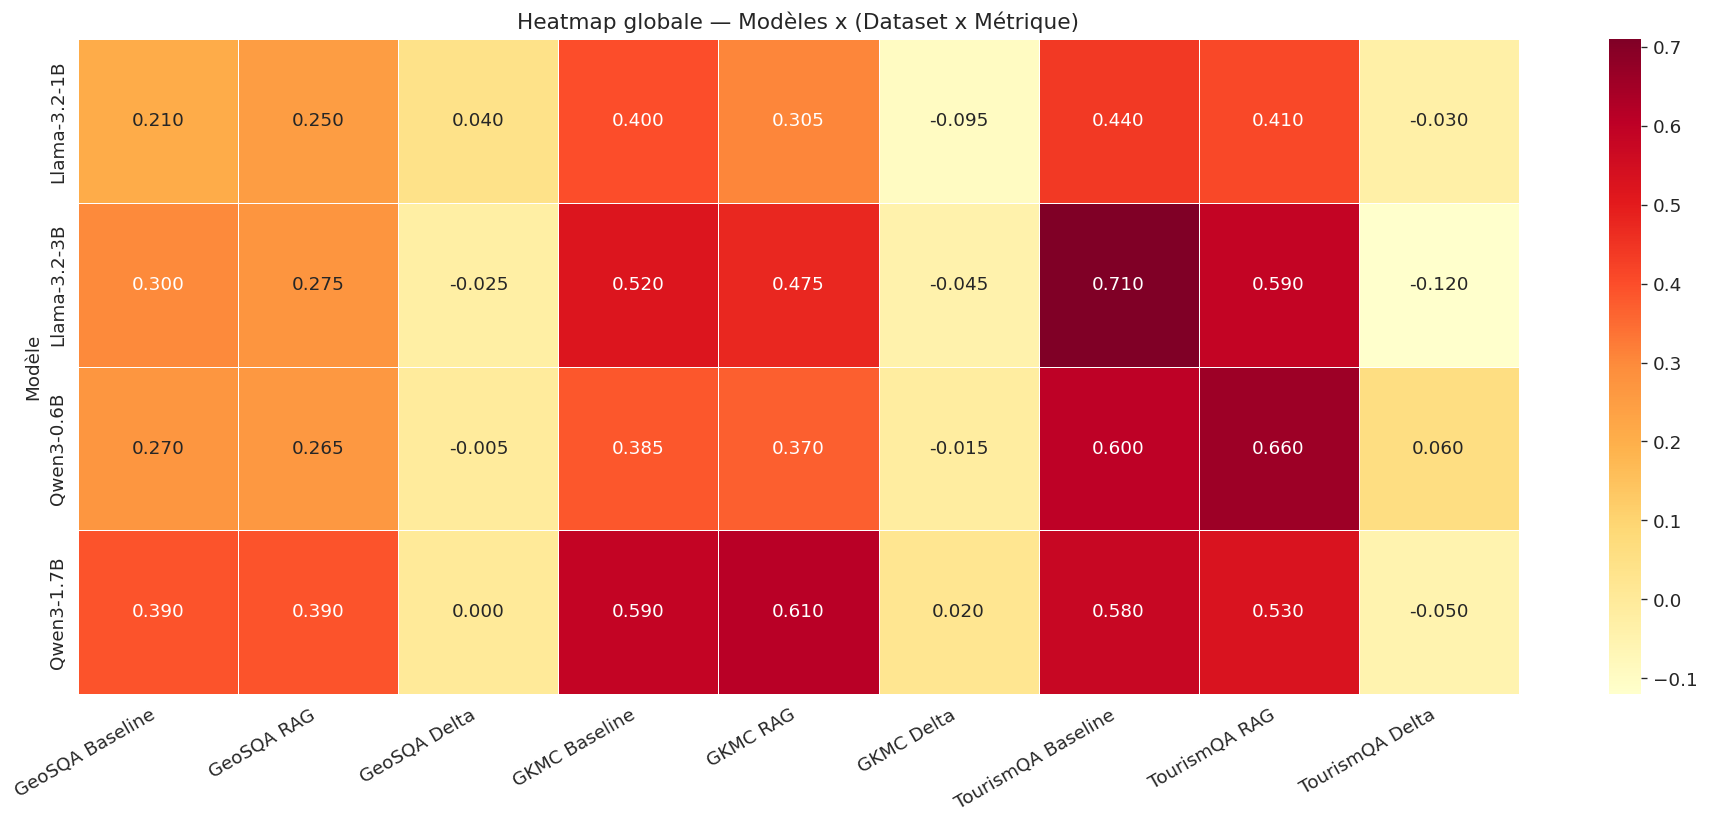
\includegraphics[width=\textwidth]{phase2d_fig6_grande_heatmap.png}
\caption{Heatmap crois\'ee --- RAG Accuracy par mod\`ele et dataset.}
\label{fig:heatmap}
\end{figure}


% ============================================================================
% 5. DISCUSSION
% ============================================================================
\section{Discussion}

\subsection{Pourquoi le RAG est-il inefficace~?}

Le r\'esultat le plus marquant de cette Phase~2 est l'impact \textbf{n\'egatif} du RAG ($\Delta$ moyen $= -0.0221$). Plusieurs facteurs expliquent ce ph\'enom\`ene~:

\begin{enumerate}[leftmargin=*]
    \item \textbf{Mismatch linguistique.} Le corpus Wikipedia est en fran\c{c}ais, tandis que les questions GeoSQA sont en anglais (traduites du chinois) et GKMC en anglais. Ce d\'ecalage rend le retriever incapable de trouver des documents pertinents (Hit Rate@5 = 0.065--0.075 pour ces deux datasets).

    \item \textbf{Contexte non pertinent.} Lorsque le retriever retourne des documents non pertinents, le contexte inject\'e dans le prompt \textbf{d\'egrade} les performances du LLM en ajoutant du bruit. Le mod\`ele doit traiter des informations inutiles qui le d\'etournent de ses connaissances internes.

    \item \textbf{Exception Tourism-QA.} Sur Tourism-QA, le corpus de reviews est en anglais (m\^eme langue que les questions) et sp\'ecifique aux POI \'evalu\'es. Le retrieval atteint un Hit Rate de 0.48, et Qwen3-0.6B b\'en\'eficie significativement du contexte ($+$0.06). Ceci confirme que le RAG fonctionne quand le corpus est linguistiquement et th\'ematiquement align\'e.
\end{enumerate}

\subsection{Pourquoi Qwen3-0.6B domine-t-il sur Tourism-QA~?}

Qwen3-0.6B, le plus petit mod\`ele, surpasse tous les autres en mode RAG sur Tourism-QA (0.6600 vs 0.5900 pour le deuxi\`eme). Deux hypoth\`eses~:

\begin{itemize}[leftmargin=*]
    \item Les mod\`eles plus grands (Llama-3.2-3B avec 0.71 en baseline) ont d\'ej\`a de bonnes connaissances internes. L'ajout de contexte RAG perturbe leur raisonnement en introduisant des informations potentiellement contradictoires.
    \item Qwen3-0.6B, ayant moins de connaissances internes, s'appuie davantage sur le contexte r\'ecup\'er\'e et en b\'en\'eficie.
\end{itemize}

\subsection{Limites de l'\'etude}

\begin{itemize}[leftmargin=*]
    \item \textbf{\'Echantillon limit\'e}~: 4~mod\`eles valides (Ministral incompatible), tous de petite taille ($\leq$3B). Les conclusions ne se g\'en\'eralisent pas n\'ecessairement aux mod\`eles plus grands (7B+).
    \item \textbf{Corpus monolingue}~: Le corpus Wikipedia en fran\c{c}ais est inadapt\'e pour des questions en anglais ou chinois. Un corpus multilingue ou en anglais am\'eliorerait le retrieval.
    \item \textbf{Variabilit\'e}~: Les r\'esultats d\'ependent de la graine al\'eatoire (seed=42), du split du dataset, et des hyperparam\`etres de g\'en\'eration.
    \item \textbf{M\'etriques h\'et\'erog\`enes}~: GeoSQA et GKMC utilisent l'accuracy MCQ, Tourism-QA utilise l'Accuracy@1 pour la recommandation. La comparaison directe entre datasets est donc approximative.
\end{itemize}


% ============================================================================
% 6. CONCLUSION
% ============================================================================
\section{Conclusion et perspectives}

\subsection{Synth\`ese}

Cette Phase~2 a \'evalu\'e 4 LLMs de petite taille sur 3 benchmarks g\'eographiques dans une configuration RAG. Les principaux r\'esultats sont~:

\begin{enumerate}[leftmargin=*]
    \item \textbf{Qwen3-1.7B est le meilleur mod\`ele global} avec une RAG Accuracy moyenne de 0.5100 sur les 3 datasets.
    \item \textbf{Le RAG est inefficace} en moyenne ($\Delta = -0.0221$), principalement \`a cause du mismatch linguistique entre le corpus (fran\c{c}ais) et les questions (anglais/chinois).
    \item \textbf{La taille du mod\`ele n'est pas corr\'el\'ee aux performances} ($r = 0.19$, non significatif). La famille Qwen surpasse syst\'ematiquement Llama.
    \item \textbf{Le retrieval fonctionne quand corpus et questions sont align\'es}~: Tourism-QA atteint un Hit Rate de 0.48 vs 0.065--0.075 pour les autres.
    \item \textbf{Qwen3-0.6B offre la meilleure efficacit\'e} (Accuracy/Taille = 0.7195), id\'eal pour le d\'eploiement sous contraintes.
\end{enumerate}

\subsection{Perspectives pour la Phase~3}

\begin{itemize}[leftmargin=*]
    \item \textbf{Corpus multilingue}~: Remplacer le corpus Wikipedia FR par un corpus en anglais ou multilingue pour \'eliminer le mismatch linguistique.
    \item \textbf{Am\'elioration du retriever}~: Tester des strat\'egies de reranking (cross-encoder) et de chunking adaptatif.
    \item \textbf{Mod\`eles plus grands}~: \'Evaluer des mod\`eles 7B+ (Qwen3-8B, Llama-3.2-8B) si les ressources GPU le permettent.
    \item \textbf{Int\'egration du meilleur mod\`ele} (Qwen3-1.7B) dans un syst\`eme RAG optimis\'e pour la Phase~3 finale.
\end{itemize}

% ============================================================================
% R\'EF\'ERENCES
% ============================================================================
\newpage
\bibliographystyle{plain}
\bibliography{../../references}

\end{document}
